\chapter{Signing System}\label{chapter:system}
In this chapter we want to describe the actual signing system, it's parts and how it works. Furthermore, this chapter includes advices how to use the system correctly and how to deploy it secure and in isolation.

\section{Idea}\label{sec:idea}
Before we start describing the system, we first want to elaborate the idea behind the system. The idea is based on the system from \citet{castle}. In their project, they had one system component that stands in an isolated glass box. The system is equipped with a monitor and a camera. Now the only channel to and from this box is an air-gapped channel based on this monitor and camera. All the data that needs to be exchanged is encoded into a QR-code and read by cameras from the screen. In \cite{castle}, the interaction with the isolated box only happens with human interaction, i.e., system administrators come and scan the QR-code from the monitor and show their own QR-codes to the system.

Unlike \cite{castle}, we use two components that do not need any human interaction except of the initialization process. The main thought here is that we use the idea of \cite{castle} to create a signing machine which is completely isolated. The second part of the system is used to receive requests from different outsiders and convert the requests to QR-codes readable by the signing component.

\begin{figure}
\centering
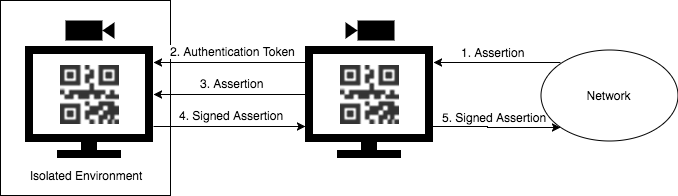
\includegraphics[width=0.8\textwidth]{images/SystemOverview.png}
\caption{This image shows a basic overview of the system components and how they interact.}
\label{fig:overview}
\end{figure}

\section{Requirements}\label{sec:requirements}
This section states the different requirements on the signing system, starting with the functional requirements followed by the non-functional requirements.

\subsection{Functional Requirements}\label{subsec:functional}
Let us start with the functional requirements of the system. The general goal of the system is to receive requests from the network containing some data. This data needs to be transfered over an air-gapped channel, signed and transfered back over the air-gapped channel and back to the network. As we have already described the idea before, this is done by using QR-codes and displaying and reading them from a screen respectively. So the system needs to be able to

\begin{enumerate}
\item receive requests from the network,
\item queue the incoming requests and handle them in \emph{first come first serve} manner,
\item encode requests in a QR-code and display the QR-code on a screen,
\item read the QR-code from a screen using a camera,
\item decode the QR-code and get its data,
\item sign the data using the \emph{Curve25519 Algorithm} \citep{bernstein2012high},
\item send the signed request back to the originating sender
\end{enumerate}

Furthermore, in order to avoid an adversary injecting some other data and getting it signed, the system needs to be able to authenticate the requests and thus only sign authenticated requests. Moreover, the system needs to be able to generate new public/private key pairs and to distribute the public keys.


\subsection{Non-Functional Requirements}\label{subse:non-functional}
After describing the functional requirements, let us concentrate on the non-functional requirements. As we have already mentioned in \autoref{sec:idea}, one part of the system needs to be isolated as much as possible. In more detail, this means

\begin{enumerate}
\item \emph{no} Internet connection,
\item \emph{no} emitting radiation (Bluetooth, WiFi, etc.),
\item \emph{no} direct connection to a power supply (in the ideal case)
\end{enumerate}

where the last point could be achieved by charging the device over induction. Furthermore, the secret/signing keys need to be kept secret and should \emph{never} leave the signing machine.

Since there is no certificate revocation in the SCION architecture \cite{scion_book} and they are using short lived certificates instead, there will be a lot of signing requests. An optimistic counting would yield in $2$ million signatures a day, which is around $23$ signatures a second. So in the ideal case, the system should be able to handle at least that amount of requests.

Moreover, in order to display and read the QR-codes, the System needs to have two screens as well as two cameras. Also, since the system is web-based as we will see in \autoref{sec:components}, the system must run on a recent browser like Google Chrome.


\section{System Components}\label{sec:components}
We have now seen the system's requirements, so let us now describe the system itself. As already mentioned in \autoref{sec:idea}, the system mainly consists of two components. This is also visible in \autoref{fig:overview}, which shows a very basic overview of the system and how the components interact with each other. There, one can see the two main components. First on the left side in the isolated environment we have the signing system, we call it the \emph{Signer}. The Signer is responsible for receiving and signing requests from the second component in the middle of \autoref{fig:overview}, which we call the \emph{Signee}. The Signee receives requests from the network and transforms the requests into readable objects for the signer. Notice here, that points 2 and 3, i.e., authentication and sending the assertion, happens in the same message (see in \autoref{fig:signee}).

In the following sections we want to describe the two components in more detail. Both components are running \texttt{Node.js}\footnote{Node.js: \url{https://nodejs.org/en/}} in version $8.6.0$. In order to read and decode the QR-codes, generate QR-codes and sign the requests, we used the following external libraries:

\begin{description}
\item[Instascan:] We used the Node module called \texttt{Instascan} from \citet{instascan} to read and decode the QR-code from a monitor. This module makes it easy to select a provided camera, e.g. the internal webcam of a laptop, and add a listener that returns the content of the QR-code once the scanner has read and decoded one.
\item[jQuery-qrcode:] Unfortunately, the Instascan module does not provide a method to generate a QR-code, so we used a plug-in for \texttt{jQuery} provided by \citet{jqueryqrcode}. This allows to use simple \texttt{jQuery}-method calls to generate a new QR-code.
\item[TweetNaCl:] In order to match the signing algorithm used in SCION \cite{scion_book}, namely the algorithm called \emph{ed25519} based on elliptic curves and introduced by \citet{bernstein2012high}, we used the Node module called \texttt{TweetNaCl} from \citet{tweetnacl}.
\end{description}


\subsection{The Signee System}\label{subsec:signee}

\begin{figure}
\centering
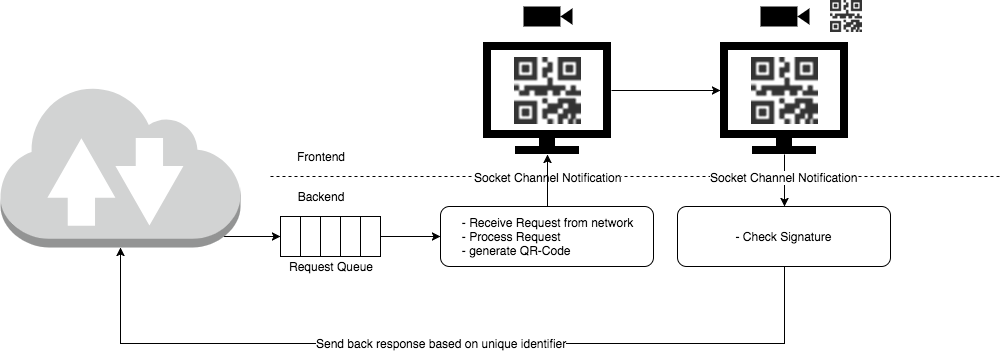
\includegraphics[width=0.8\textwidth]{images/Signee.png}
\caption{This figure shows a general overview of the \emph{Signee}}
\label{fig:signee}
\end{figure}

In this section we want to describe the first part of the system that a request reaches, namely the \emph{Signee}. The Signee listens on a predefined port (default port is $3000$) for \texttt{POST} requests containing data that needs to be signed by the \emph{Signer}. Thereby, the request needs to have the following parameters:

\begin{code}[caption={Expected message format when sending a new request to the Signee}]
data=DATA_TO_SIGN&from=VALID_FROM&to=VALID_TO
\end{code}

where DATA\_TO\_SIGN stands for the actual data that needs to be signed by the Signer, for example an assertion for a name resolution. The parameters $from$ and $to$ describe the desired validity range. Notice, that it is the desired validity range and that the Signer checks whether it is a valid range or not (more on this later).

Once a request is received, the Signee puts it in a queue, together with a callback to a request handler. Every request in the queue is then handled in \emph{first in first out} (FIFO) order. In order to hinder an adversary to inject any irregular request, every request gets authenticated by appending the \texttt{HMAC} of the data to the request. We use the \texttt{HMAC} module from the Node.js crypto library\footnote{Node.js Crypto Library: \url{https://nodejs.org/api/crypto.html}} to achieve this. The request is then sent to the front-end, i.e., the browser, using \emph{Socket Notifications}. Notice that the system expects a specific \texttt{JSON} format like in \autoref{listing:signee_to_signer}. Moreover, notice the unique identification number. This identification number is computed by calculating the hash of the request. The ID is used to reference back to the original request such that the Signee is able to return to the right requester later on.

\begin{code}[caption={Expected message format from the Signee to the Signer}, label={listing:signee_to_signer}]
{
    id: UNIQUE_ID,
    data: { data: DATA_TO_SIGN,
            from: VALID_FROM,
            to: VALID_TO },
    mac: HMAC_OF_DATA
}
\end{code}

The browser then encodes this information into a QR-code using the \emph{jQuery plug-in} mentioned before.

Once the Signee scans a new QR-code from the Signer's screen, the browser decodes it and sends the decoded content back to the back-end again using \emph{Socket Notifications}. The Signee then checks whether the signature is indeed from the expected Signer and if yes, it sends the signed data back to its origin. In order to handle the right request and response objects, the Signee uses the unique id which it has computed before. The final response has the format like in \autoref{listing:signee_to_origin}.

\begin{code}[caption={Expected message format from the Signee back to the origin}, label={listing:signee_to_origin}]
{
    assertion: { data: DATA_TO_SIGN,
                 valid_from: DATE_IN_UTC_FORMAT,
                 valid_until: DATE_IN_UTC_FORMAT },
    signature: SIGNATURE_OF_ASSERTION
}
\end{code}

You can find a graphical overview of the Signee in \autoref{fig:signee}. This overview shows the very high-level interaction between the front-end and the back-end of the Signee.


\subsection{The Signer System}

\begin{figure}
\centering
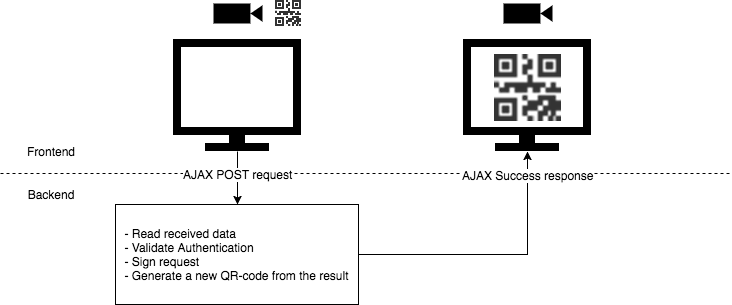
\includegraphics[width=0.8\textwidth]{images/Signer.png}
\caption{This figure shows a general overview of the \emph{Signer}}
\label{fig:signer}
\end{figure}

After having covered the Signee, we now want to describe the second component of the system, namely the \emph{Signer}. Similar to the Signee, the Signer runs a Node.js server. However, unlike the Signee, the Signer gets its requests not from the network, but reads it from the Signee's screen. One reason for this is the requirement that the Signer needs to be totally isolated and therefore can not be connected to any network. In order to read the QR-code from the Signee's screen, the Signer also uses the Instascan module as described before. Once the QR-code has been read and decoded by the module, the content is sent to the back-end using an \texttt{AJAX POST request}. The back-end first verifies the authentication token, i.e., checking the hash of the data against the received hash-value. If it is correct, the Signer extracts the data from the request and checks the validity range. Thereby, the starting date must start in the future and the duration must not be longer than a predefined maximum value. If the validity range is valid, the Signer signs the data together with the validity range.

\begin{code}[caption={Expected message format from the Signer back to the Signee}, label={listing:signer_to_signee}]
{
    id: UNIQUE_ID,
    assertion: { data: DATA_TO_SIGN,
                 valid_from: DATE_IN_UTC_FORMAT,
                 valid_until: DATE_IN_UTC_FORMAT },
    signature: SIGNATURE_OF_ASSERTION },
}
\end{code}

The result is then sent back to the front-end using success callback of the \texttt{AJAX} request using the format in \autoref{listing:signer_to_signee}. In the front-end, the response is encoded into a QR-code and displayed on the screen for the Signee to read it. The important part here is that the Signer sends back the request identifier so that the Signee can redirect the signed data to the right originator. 

\autoref{fig:signer} shows a graphical overview of the interaction between the front-end and the back-end of the Signer.

\section{System Setup}\label{sec:setup}
Now that we have described the two system components, we want show our prototype setup. For our prototype setup we first met the assumption of complete isolation of the Signer system, i.e., we did not especially shield or isolate the system. However, we argue that since the system implementation does not need any Internet connection or some other connection, we could simply use the method of \cite{castle} in order to make the Signer running in an isolated environment.

% TODO: name specific laptop specification
The overall system setup is very minimalistic. For each of the two components we simply used a commodity laptop. For the Signer we used a HP Aspire and for the Signee a Lenovo Thinkpad. Both laptops run a clean install of Ubuntu $16.04.3$ LTS with the Google Chrome Browser and Node.js Server installed additionally.

\subsection{Initialization}
Before the system is ready to run correctly, both components need first to be initialized. The initialization includes downloading the corresponding source code and then in a next step installing the needed \emph{node-modules}. The best way to do this is to simply run \texttt{npm install}. Notice that one will need the \texttt{package.json} file (see \autoref{listing:package_json}) from the repository\footnote{GitHub Repository: \url{https://github.com/fmurer/master_thesis}}.

\begin{code}[caption={Example \texttt{package.json} containing the needed node-modules}, label={listing:package_json}]
{
  "name": "signer",
  "version": "1.0.0",
  "description": "",
  "main": "app.js",
  "scripts": {
    "test": "echo \"Error: no test specified\" && exit 1"
  },
  "author": "Fabian Murer",
  "license": "ISC",
  "dependencies": {
    "express": "^4.16.2",
    "jquery": "^3.2.1",
    "morgan": "^1.9.0",
    "node-schedule": "^1.2.5",
    "qrcode-generator": "^1.3.1",
    "socket.io": "^2.0.4",
    "tweetnacl": "^1.0.0"
  }
}
\end{code}

Next to installing the modules from \texttt{package.json}, one also needs to install \emph{Instascan} \cite{instascan} and the \emph{jQuery plug-in} \cite{jqueryqrcode} for generating the QR-codes. Furthermore, a system administrator needs to place the Signer's public key on the Signee before starting the system, otherwise the Signee fails to verify the responses from the Signer. For the initial key generation, a script is provided (see \autoref{listing:key_gen}). So the administrator only needs to put the file \texttt{signer.pub} onto the Signee.

\begin{code}[language=bash, breaklines=true, caption={Script for initial key pair generation}, label={listing:key_gen}]
#!/bin/bash

keypair="$(node -e 'keyPair = require("../signer/node_modules/tweetnacl").sign.keyPair();
console.log(Buffer.from(keyPair.publicKey).toString("hex"));
console.log(Buffer.from(keyPair.secretKey).toString("hex"));
console.log("");')"

echo "${keypair}"

counter=0
while IFS='' read -r line || [[ -n "$line" ]]; do
	echo "$line" > key_"$counter"
	let counter++
done <<< "${keypair}"

mv ./key_0 ../signer/pk/signer.pub
mv ./key_1 ../signer/sk/sign_key
\end{code}

After having installed all the needed modules, the system administrator should also manually launch the pairing of the systems by pressing the $p$ button on the Signee's keyboard. This guarantees an initial shared secret between the Signer and the Signee which is then used for authenticating the messages sent from the Signee to the Signer.


\subsection{Running Example}
Once everything is initialized according to what we have seen before, the rest of the setup is really simple. The two laptops need to be placed opposed to each other such that the camera of the Signee can see the monitor of the Signer and vice versa.

\begin{description}
\item[Remark:] \textit{One thing that came across while implementing and testing the system was that a too bright monitor makes the camera unable to read the QR-code from it, because the white parts outshine the dark parts. So in order for the cameras to read properly, the brightness needs to be adjusted accordingly. In the current setup with the two laptops, this means reducing the screen brightness to maximum $50\%$.}
\end{description}

This is already all for a basic example. The only thing left is to start both servers with \texttt{node app.js}. Now one can send \texttt{POST} requests using the format mentioned in \autoref{subsec:signee} and send it to the Signee on the specific port (default is port $3000$). \autoref{fig:prototype} shows a running example including a view on the monitors.

\begin{figure}
\centering
%\includegraphics[width=0.8\textwidth]{}
\caption{Example setup of the prototype showing the monitors while running}
\label{fig:prototype}
\end{figure}







